\chapter[SID]{SID}
--------------------- FALAR SOBRE O SID

\section{Visão Geral}
O SID está estruturado em duas possíveis vertentes, o WEB e o \textit{mobile}, ele foi desenvolvido com o objetivo de oferecer uma forma mais intuitiva, dinâmica e amigável para o administrador e para o usuário do sistema. Atendendo ao objetivo principal, onde é divulgação de informações através de uma plataforma WEB e \textit{mobile}.

Necessitando sempre do uso da rede para realizar atualizações, o SID está dividido em três módulos, o primeiro deles é o administrador, onde é possível fazer o gerenciamento completo do conteúdo que será apresentado no segundo modulo, no caso o módulo cliente, nesse segundo módulo será apresentado as informações que foram cadastradas no módulo
administrador e serão propagadas por monitores ou celulares. O terceiro módulo não é acessível, ele é encarregado de fazer toda recuperação dos dados que será apresentada na vertente WEB e \textit{mobile}.

A arquitetura cliente-servidor mostrou-se necessário para minimizar o processamento do cliente, centralizando o processamento das informações em um sistema mais robusto.

O administrador é responsável por gerenciar todas as informações do sistema, inserindo, alterando, e retirando as divulgações, ou seja, faz o gerenciamento das informações a serem repassadas ao módulo cliente ou \textit{mobile} que, por sua vez, de forma simples, o cliente tem apenas o trabalho de apresentar as divulgações de maneira atrativa e dinâmica, enquanto o \textit{mobile} é responsável por apresenta as divulgações e fornece a possibilidade de troca de mensagens entre professores e alunos. 


--------------- FALAR SOBRE COMO O SID FOI DESENVOLVIDO

\section{Modulo Administrador}
 \begin{enumerate}
   \item Legenda: É um campo de texto destinado a informação a ser repassada de forma sucinta e clara ao usuário final por intermédio cliente ou mobile. 
   \item Texto: É todo o texto que será enviado ao Facebook, contendo informações como descrição da publicação, data e horário da realização e um possível \textit{link} para acesso a mais informações. 
   \item Data de Início: É a data inicial em que o publicação começará a ser exibida no cliente e no mobile.
   \item Data de Término: É a data final em que o publicação deixará de ser exibida no cliente e no mobile.
   \item Imagem: Será a imagem enviada para o Facebook, para o cliente e para o mobile. Essa imagem pode ser um \textit{banner} de apresentação de um evento, por exemplo.
 \end{enumerate}
 
 ------ MUDAR NUMERO DAS FIGURAS!
 
 A Figura 2, consiste em representar como os elementos supracitados são inseridos a partir da visão do operador do sistema no módulo administrador. O diagrama de sequência para esta funcionalidade encontra-se na Figura 10.

 
 \begin{figure}[!htb]
\centering
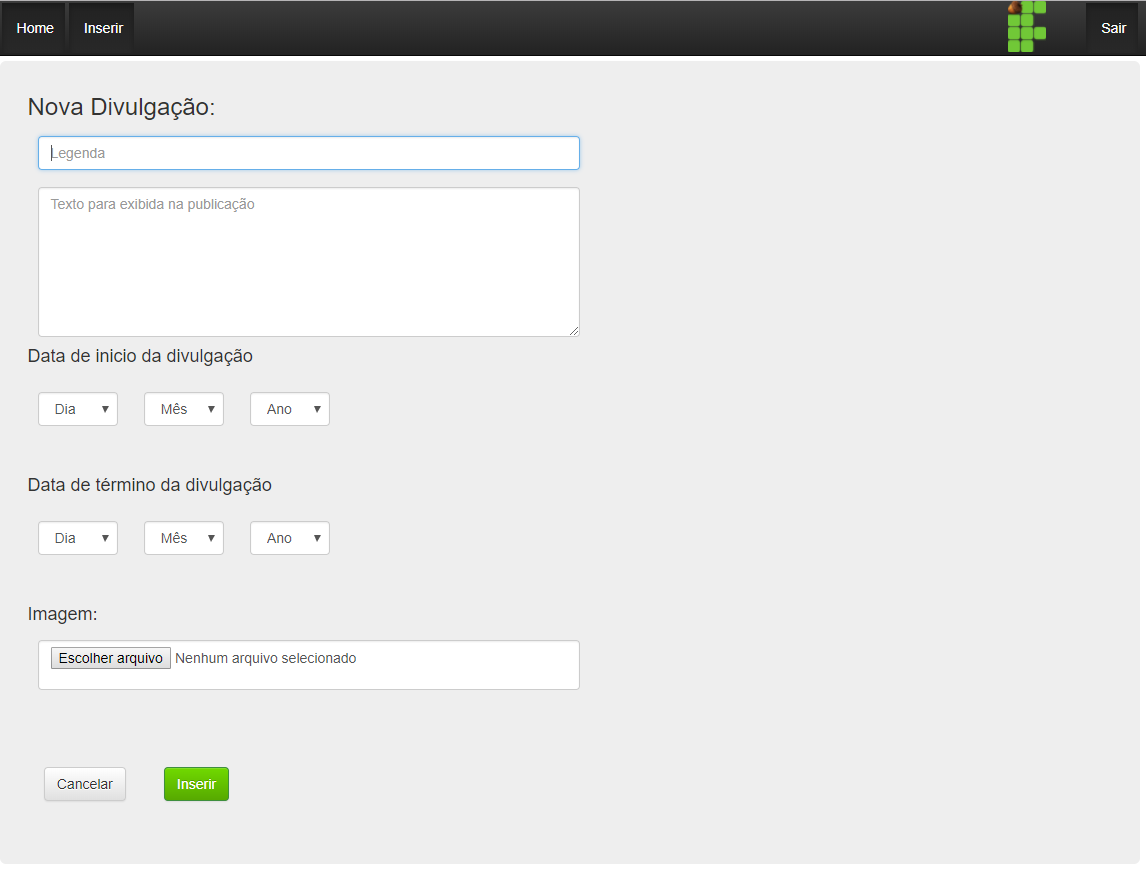
\includegraphics[scale=0.6]{figuras/administrador1}
\caption{Página de inserção no módulo administrador.}
\label{Rotulo}
\end{figure}

-- ESCREVER MAIS

\section{Modulo Cliente}
-- FALAR SOBRE

 ------------- MUDAR IMAGEM
\begin{figure}[!htb]
\centering
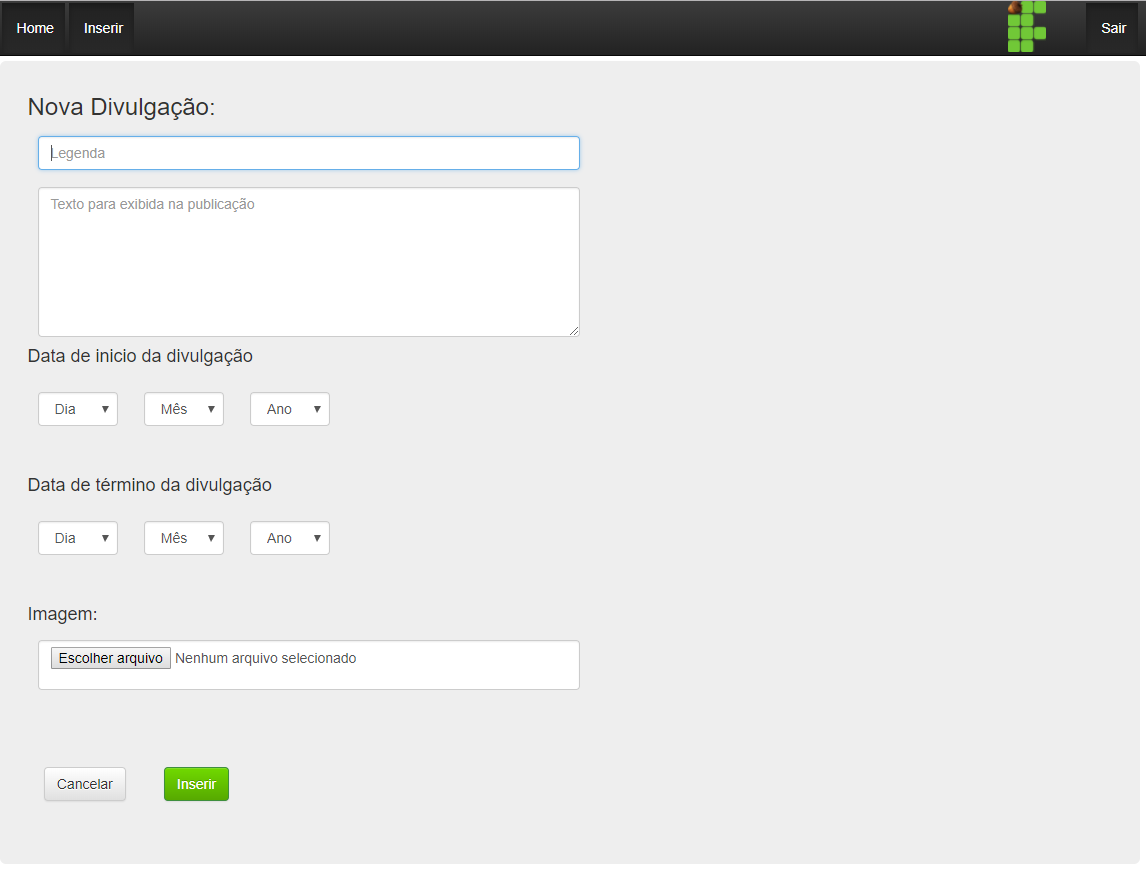
\includegraphics[scale=0.6]{figuras/administrador1}
\caption{Página de inserção no módulo administrador.}
\label{Rotulo}
\end{figure}

\section{Modulo API}
\section{Arquitetura}
------ COLOCAR DIAGRAMA DE CLASSES

------ COLOCAR CASOS DE USO

------ COLOCAR DIAGRAMA DE SEQUENCIA
 

\section{Possível solução para Implementação - Rapberry}
Desde a sua invenção em 1971, microprocessadores vem sendo usados no desenvolvimento dos mais variados tipos de eletrônicos ou outros equipamentos, substituindo até mesmo sistemas mecânicos. Algo que vai além de um simples software, os microprocessadores devem ser capazes controlar as ações de um dispositivo. \cite{rosenstark2007}

Para \cite{aristotelous2016}, o objetivo essencial de todos os tipos de empresa é a rentabilidade, podendo ela ser alcançada usando uma solução de baixo custo, boas tecnologias e com um preço atrativo. Teste do \cite{aristotelous2016} apresenta a possibilidade de se ter um servidor completamente funcional com sistema operacional Linux por um equipamento de 35\$, possibilitando a criação de um servidor, por exemplo de um repositório na nuvem com um baixo custo, flexibilidade e eficiência energética. 

Grandes servidores oferecem um melhor desempenho, entretanto, o baixo uso, a pouca eficiência energética ou até mesmo o pouco espaço podem limitar o uso desse tipo de equipamento. Nesse sentido, para \cite{cusick2014}, placas de circuito oferecem vantagens como o uso de pouco espaço, desempenho significante com baixo custo e consumo, além do suporte a diversas soluções de software oferecendo múltiplas opções de interface com uma variante do Linux. 